\documentclass{article}\usepackage[]{graphicx}\usepackage[]{color}
%% maxwidth is the original width if it is less than linewidth
%% otherwise use linewidth (to make sure the graphics do not exceed the margin)
\makeatletter
\def\maxwidth{ %
  \ifdim\Gin@nat@width>\linewidth
    \linewidth
  \else
    \Gin@nat@width
  \fi
}
\makeatother

\definecolor{fgcolor}{rgb}{0.345, 0.345, 0.345}
\newcommand{\hlnum}[1]{\textcolor[rgb]{0.686,0.059,0.569}{#1}}%
\newcommand{\hlstr}[1]{\textcolor[rgb]{0.192,0.494,0.8}{#1}}%
\newcommand{\hlcom}[1]{\textcolor[rgb]{0.678,0.584,0.686}{\textit{#1}}}%
\newcommand{\hlopt}[1]{\textcolor[rgb]{0,0,0}{#1}}%
\newcommand{\hlstd}[1]{\textcolor[rgb]{0.345,0.345,0.345}{#1}}%
\newcommand{\hlkwa}[1]{\textcolor[rgb]{0.161,0.373,0.58}{\textbf{#1}}}%
\newcommand{\hlkwb}[1]{\textcolor[rgb]{0.69,0.353,0.396}{#1}}%
\newcommand{\hlkwc}[1]{\textcolor[rgb]{0.333,0.667,0.333}{#1}}%
\newcommand{\hlkwd}[1]{\textcolor[rgb]{0.737,0.353,0.396}{\textbf{#1}}}%

\usepackage{framed}
\makeatletter
\newenvironment{kframe}{%
 \def\at@end@of@kframe{}%
 \ifinner\ifhmode%
  \def\at@end@of@kframe{\end{minipage}}%
  \begin{minipage}{\columnwidth}%
 \fi\fi%
 \def\FrameCommand##1{\hskip\@totalleftmargin \hskip-\fboxsep
 \colorbox{shadecolor}{##1}\hskip-\fboxsep
     % There is no \\@totalrightmargin, so:
     \hskip-\linewidth \hskip-\@totalleftmargin \hskip\columnwidth}%
 \MakeFramed {\advance\hsize-\width
   \@totalleftmargin\z@ \linewidth\hsize
   \@setminipage}}%
 {\par\unskip\endMakeFramed%
 \at@end@of@kframe}
\makeatother

\definecolor{shadecolor}{rgb}{.97, .97, .97}
\definecolor{messagecolor}{rgb}{0, 0, 0}
\definecolor{warningcolor}{rgb}{1, 0, 1}
\definecolor{errorcolor}{rgb}{1, 0, 0}
\newenvironment{knitrout}{}{} % an empty environment to be redefined in TeX

\usepackage{alltt}
\graphicspath{{../inst/results/}}


%%% PACKAGES
\RequirePackage{hhline}
\RequirePackage{graphicx}
\RequirePackage{mathtools, amsmath, amsfonts, amsthm, amssymb}
\RequirePackage{mdwlist}
\RequirePackage{booktabs}
\RequirePackage{setspace}
\RequirePackage{tikz}
\RequirePackage{pgf}
\RequirePackage[utf8]{inputenc} 
\RequirePackage{multirow}
\RequirePackage{booktabs} 				% for much better looking tables
\RequirePackage{array} 					% for better arrays (eg matrices) in maths
\RequirePackage{paralist} 				% very flexible & customisable lists (eg.
                                        % enumerate/itemize, etc.)
\RequirePackage{verbatim} 				% For ommenting out blocks of text 
\RequirePackage{subfig} 				% For including more than one captioned
                                        % figure/table in a single float
\RequirePackage{hyperref}				%For clickable references
\RequirePackage{scrextend}				%For paragraph indenting
\RequirePackage[sort&compress]{natbib}	%For citations 
\RequirePackage{titlesec}				% Customizes section headings
\RequirePackage{ellipsis}
\RequirePackage{grffile}


%%% PRELIMINARY COMMANDS FOR VIGNETTE
\makeatletter
%\VignetteIndexEntry{Positivity violations}
%\VignetteKeywords{positivity, longitudinal, causality}
%\VignettePackage{positivity}
%\VignetteEngine{knitr::knitr}
\makeatother


%%% PAGE DIMENSIONS
\RequirePackage{geometry} % to change the page dimensions
\geometry{letterpaper} % or letterpaper (US) or a5paper or....
\geometry{margin=1in} % for example, change the margins to 2 inches all round
% \geometry{landscape} % set up the page for landscape
% read geometry.pdf for detailed page layout information


%%% HEADERS & FOOTERS
\usepackage{fancyhdr} % This should be set AFTER setting up the page geometry
\pagestyle{fancy} % options: empty , plain , fancy
\renewcommand{\headrulewidth}{1pt} % customise the layout...
\lhead{\textsc{Tran} et al.}
\chead{}
\rhead{January 2015}
\lfoot{}
\cfoot{\thepage}
\rfoot{}


%%% SECTION TITLE APPEARANCE
\RequirePackage{sectsty}
\allsectionsfont{\bfseries\rmfamily} % (See the fntguide.pdf for font help)
\subsectionfont{\bfseries\fontsize{12}{12}\rmfamily}
\subsubsectionfont{\bfseries\fontsize{11}{11}\rmfamily}
% (This matches ConTeXt defaults)


%%% ToC (table of contents) APPEARANCE
\usepackage[nottoc,notlof,notlot]{tocbibind} % Put the bibliography in the ToC
\usepackage[titles,subfigure]{tocloft} % Alter the style of the Table of Contents
\renewcommand{\cftsecfont}{\rmfamily\mdseries\upshape}
\renewcommand{\cftsecpagefont}{\rmfamily\mdseries\upshape} % No bold!
\newcommand{\indep}{\rotatebox[origin=c]{90}{$\models$}}


%%% CUSTOMIZED COMMANDS 
\renewcommand{\indent}{\hskip 20pt}
\newcommand{\pdot}{\mkern-2mu\cdot\mkern-2mu} 
\newcommand{\E}{\mathbb{E}}
\newcommand{\I}{\mathbb{I}}
\newenvironment{eq}{\equation\nonumber}{\endequation}

%%% END Article customizations

%%%%%%%%%%%%%%%%%%%%%%%%%%%%%%%%%%%%%%%%%%%%%%%%%%%%%%%%%%%%%%%%%%%%%%%%%%%%%%%
%%%%%%%%%%%%%%%%%%%%%%%%%%%%%%%%%%% TITLE %%%%%%%%%%%%%%%%%%%%%%%%%%%%%%%%%%%%%
%%%%%%%%%%%%%%%%%%%%%%%%%%%%%%%%%%%%%%%%%%%%%%%%%%%%%%%%%%%%%%%%%%%%%%%%%%%%%%%
\title{Handling positivity violations in longitudinal data}
\author{Linh Tran \\
		Maya Petersen \\
        Mark van der Laan \\
		et al.}
\date{January 5, 2015}
\IfFileExists{upquote.sty}{\usepackage{upquote}}{}
\begin{document}
%\SweaveOpts{concordance=TRUE}
\maketitle




%%%%%%%%%%%%%%%%%%%%%%%%%%%%%%%%%%%%%%%%%%%%%%%%%%%%%%%%%%%%%%%%%%%%%%%%%%%%%%%
%%%%%%%%%%%%%%%%%%%%%%%%%%%%%%%%%% ABSTRACT %%%%%%%%%%%%%%%%%%%%%%%%%%%%%%%%%%%
%%%%%%%%%%%%%%%%%%%%%%%%%%%%%%%%%%%%%%%%%%%%%%%%%%%%%%%%%%%%%%%%%%%%%%%%%%%%%%%
\begin{abstract}

The abstract goes here.

\end{abstract}


%%%%%%%%%%%%%%%%%%%%%%%%%%%%%%%%%%%%%%%%%%%%%%%%%%%%%%%%%%%%%%%%%%%%%%%%%%%%%%%
%%%%%%%%%%%%%%%%%%%%%%%%%%%%%%%%% BACKGROUND %%%%%%%%%%%%%%%%%%%%%%%%%%%%%%%%%%
%%%%%%%%%%%%%%%%%%%%%%%%%%%%%%%%%%%%%%%%%%%%%%%%%%%%%%%%%%%%%%%%%%%%%%%%%%%%%%%
\section{Introduction}

\indent Background goes here...
\newline

\indent The use of causal estimators have become very popular in many fields,
from statistics, to the social sciences, to economics. Estimators developed
under this framework benefit by combining both the estimation of parameters from
a statistical model and causal inference under non-testable assumptions of randomization and
positivity. One well known approach for the estimation of these
parameters is the inverse probability of treatment weighted (IPTW) estimator. As
an estimating equation based estimator the the conditional probability of
treatment is required. Normally estimated from the empirical distribution,
these propensity scores calculated can then be used in a working marginal
structural model, projecting the true dose response curve onto a parametric
model. This powerful approach has further been expanded to a longitudinal
setting where time dependent confounding may exist. In this setting, a covariate
can simultaneously act as both a confounder and as an intermediate. Because bias
is introduced by controlling for a variable affected by treatment, more standard
classical methods cannot be applied. The longitudinal IPTW avoids this and
allows us to control for confounding in an unbiased approach to the estimation
of our causal parameter.
\newline

\textcolor{red}{define positivity.} Valid estimation of these causal parameters
rely on three primary assumptions. Consistency assumes that if the treatment is $A=a$ for a given
subject, then $Y_a=Y$. This assumption is sometimes known as the counterfactual
outcome since it is assumed that under specific treatment regimes, the potential
(but unrealized) outcome would equal the observed outcome. Conditional
exchangeability (aka the randomization assumption) assumes that there is no
unmeasured confounding given data on the covariates $L$ (i.e. $Y_a \coprod A|L$
for all possible values of $a$ and $\ell$). Lastly, positivity assumes that if
$f_L(\ell) \neq 0$, then $f_{A|L}(a|\ell)>0$ for all $a$, where
$f_L(\ell) \equiv P(L=\ell)$ is the population marginal probability that $L$
takes the value $\ell$ and $f_{A|L}(a|\ell) \equiv P(A=a|L=\ell)$ is the
conditional probability that $A$ takes the value $a$ among subjects in the population where $L=\ell$
\cite{Robins:ch23}. We define this assumption formally as
\begin{equation}
	\underset{a \in \mathcal{A}}{\inf}P_0(A=a|L)>0 \text{ a.e.}
\end{equation}
where $\mathcal{A}$ is the set of all possible counterfactual treatments. This
assumption of positivity is particularly important for IPTW estimators, as these
estimators are very sensitive to positivity violations as well as near
violations.
\newline

\textcolor{red}{Talk about how positivity can arise} In realistic clinical care
settings, monitoring times can (a) determine the time points at which treatment 
can change (and are thereby are a source of
positivity violation for some treatment regimens), (b) affect the outcome
directly (and are also thereby confounders), and (c) affect when data on a given
individual are observed (and thereby the plausibility of the sequential
randomization assumption (SRA)). Thus we are faced with a situation where not
only is positivity an issue, but that the covariate causing the positivity acts as a
confounder and can single handedly threaten the conclusions of our study. In
estimating treatment specific counterfactuals, it is required that very careful
consideration of both the counterfactual parameter of interest and the
positivity violations be given.
\newline

\textcolor{red}{Talk about example we'll work with} For example, consider the
problem in which longitudinal clinical data including clinic visits, time
updated CD4 count, and mortality are measured on a sample of HIV patients
starting at time of virologic failure of first line antiretroviral therapy
(ART). The question of interest is whether a delay in switching off failing ART
onto a secondary medication affects mortality.
That is, we aim to use data of the described form to estimate how the
counterfactual survival or hazard varies as a function of assigned
switch time. While some patients may come in to visit frequently, we are faced
the inevitability that others will not. It is obvious that for patients that do
not come in for clinical visits, the probability of switching off failing ART is
0. We therefore have a serious positivity violation. Additionally, patients who
come in more often may have better quality of care, thus affecting the outcome
of interest. We also are unable to measure important confounders such as the
time updated CD4 count. \textcolor {red} {continued...} As a working example for
the present paper, we consider a population of subjects with HIV who have failed their primary antiretroviral (ARV) therapy
medication. Among these subjects, we are interested in analyzing whether
switching to secondary medication results in reduced mortality. More
specifically, we are interested in determining whether delays in switching to
secondary medication result in different mortality rates. For example,
do subjects who switch medication immediately after primary ARV failure
experience lower mortality than those who switch at a later time point?
\newline

In this paper we use simulations to demonstrate the bias involved if
monitoring is either excluded from the adjustment set (due to confounding) or
is included (due to positivity). We then demonstrate each of the possible
alternatives presented above. Section \ref{sec:data} formally defines the data,
our statistical and causal model, and discusses identifiability.
Section \ref{sec:parameters} presents details on each of our approaches,
including the exact parameters being estimated. Section \ref{sec:simulation}
investigates the bias incurred by mishandling the monitoring covariate and the
performance of each approach presented. Section \ref{sec:discussion} concludes
with some remarks about each of the approaches and advocates for a systematic
approach to addressing potential violations in positivity.

We then simulate data such that the positivity violation is present and
demonstrate the performance of each approach under this known true probability distribution. 



%%%%%%%%%%%%%%%%%%%%%%%%%%%%%%%%%%%%%%%%%%%%%%%%%%%%%%%%%%%%%%%%%%%%%%%%%%%%%%%
%%%%%%%%%%%%%%%%%%%%%%%%%%%%%%%%% PROPOSALS %%%%%%%%%%%%%%%%%%%%%%%%%%%%%%%%%%%
%%%%%%%%%%%%%%%%%%%%%%%%%%%%%%%%%%%%%%%%%%%%%%%%%%%%%%%%%%%%%%%%%%%%%%%%%%%%%%%
\section{Positivity approaches}
\label{sec:proposals}

\indent In response to the positivity violations presented above, we propose
several approaches that either target parameters not affected by the violation or
modify the target parameter such that there is appropriate support for
estimation. 

\subsection{Selecting appropriate interventions}

\indent One can limit the static treatment regimes of interest to only those for
which no positivity violations occur. For example, one might simply contrast mortality
under a regime that forces patients to switch immediately with one that says
never switch. Furthermore, a reasonable approach could be to assume linearity in
the dose response curve and to interpolate between the two estimates. 

\subsection{Dynamic regimes}

\indent One might redefine the intervention as a "realistic" dynamic regime. In
our example, the intervention of interest would have an assigned switch time, and
then force a subject to switch at the first time point he or she is seen after
his assigned time.

\subsection{Joint interventions}

\indent One might chose to intervene jointly on the monitoring times and the
treatment (i.e. switch time). We note that whereas the latter two approaches leave the
monitoring time to be random, this approach additionally intervenes on the
monitoring mechanism itself. This monitoring intervention is less restrictive
than, say, forcing patients to come in for clinical visits at all time points,
as it forces a patient to come in only at time t during which the patient is
forced to switch to secondary medication.

\subsection{Excluding covariates}

\indent A potential approach is to simply ignore the covariate causing the
positivity violation. While this avoids the issue, it can result in noticeable bias
depending on whether the covariate directly affects the outcome of interest.


%%%%%%%%%%%%%%%%%%%%%%%%%%%%%%%%%%%%%%%%%%%%%%%%%%%%%%%%%%%%%%%%%%%%%%%%%%%%%%%
%%%%%%%%%%%%%%%%%%%%%%%%%%%%%%%% SIMULATIONS %%%%%%%%%%%%%%%%%%%%%%%%%%%%%%%%%%
%%%%%%%%%%%%%%%%%%%%%%%%%%%%%%%%%%%%%%%%%%%%%%%%%%%%%%%%%%%%%%%%%%%%%%%%%%%%%%%
\section{Simulations}

\indent We approach our simulation under discrete time points in which a subject
cannot experience an event in between time $t$ and $t+1$. Subjects are followed up to
a fixed time point $K+1$, at which point it is observed whether or not
they have experienced an failure. Let our observed data be denoted as
\begin{equation}
  O = (L(0), A(0), L(1), A(1), \ldots, L(K), A(K), Y = L(K+1))
\end{equation}
where $L(t)=(Y(t), L1(t), L2(t))$, $A(t)=(Z(t), A1(t))$, and $L(0)$ also
includes $(W1,W2)$. We describe each of the covariates for the simulation below.

\begin{itemize*}
    \item $W1$ is a baseline continuous covariate.  
    \item $W2$ is a baseline bernoulli covariate. 
	\item $Y(t)$ is an indicator of an event. As a counting process, it jumps to
	and remains at 1 once a subject experiences a failure.
    \item $L1(t)$ is a time-varying continuous covariate. 
    \item $L2(t)$ is a time-varying continuous covariate. 
    \item $Z(t)$ is an indicator that the subject has a clinical visit. 
    \item $A1(t)$ is an indicator that the subject switches to
    secondary medication. As a counting process, this covariate also jumps to
    and remains at 1 once a subject switches medication. 
\end{itemize*}

For the present simulation, the true probability distribution is defined
through each individual covariate as a process dependent upon $t$. That is, we
define each covariate to follow the distribution

\begin{itemize*}
    \item $W1 \sim N(0,1)$
    \item $W2 \sim Ber(logit^{-1}(.2))$
    \item $L1(t) \sim N(0.1 + 0.4\pdot W1 + 0.6\pdot L1(t-1) - 0.7\pdot L2(t-1) - 0.45\pdot A1(t-1), 0.5^{2})$
    \item $L2(t) \sim N(-0.55 + 0.5\pdot W1 + 0.75\pdot W2 + 0.1\pdot L1(t-1) + 0.3\pdot L2(t-1) - 0.75\pdot A1(t-1), 0.5^{2})$
    \item $Z(t) \sim Ber(logit^{-1}(2.8 - 0.5\pdot W1 + 0.6\pdot W2 + 0.7\pdot L1(t) + 0.7\pdot L2(t)))$
    \item $A1(t) \sim Ber(logit^{-1}(-1.5 - 1.5\pdot W1 + 0.75\pdot W2 + 0.8\pdot L1(t) + 0.8\pdot L2(t))), \text{ if } A(t-1)=0 \text{ \& } Z(t)=1$
    \item $Y(t) \sim Ber(logit^{-1}(-1.8 + 1.2\pdot W1 - 2.4\pdot W2 - 1.6\pdot L1(t-1) - 1\pdot L2(t-1) - 1.9\pdot A1(t-1) - \beta_{Z}\pdot Z(t-1)))$
\end{itemize*}

where once $Y(t)=1$, all remaining covariate values become degenerate and are
defined as the last value carried forward with probability 1. We define
$A1(t)$ such that if $A(t-1)=1$ or $Z(t)=0$ then $A(t)=A(t-1)$. Additionally,
at time $t=0$, all covariate values at $t-1$ are set to be $0$. We note that
under this model, $A1(t)$ is defined to have a large beneficial effect on the
outcome $Y(t)$. That is, observations with $A1(t)=1$ at lower time points $t$
will have a noticeably lower probability of event $Y(t)$ than those with $A1(t)=0$. 
\newline 

To analyze how severely option \#4 (i.e. ignoring the causing the positivity
violation) affects estimates of our target parameter, we undertake two
simulations under this specified model, with either $\beta_Z = 1.25$ or $\beta_Z
= 0$. The former $\beta_Z$ accounts for the scenario that clinical visits
directly affect the outcome, whilst the latter defines no direct effect on the
outcome.

\subsection{Target parameter}

\indent Formally, a parameter is defined as a mapping $\Psi$ which can be
applied to any probability distribution $P$. The range for this mapping is
the parameter space, normally considered to be the real number line
$\mathbb{R}$. Here, we define this mapping to be 
\begin{equation}
\Psi(P_0^{\bar{a}}) \equiv  \mathbb{E}_{P_0^{\bar{a}}}Y.
\end{equation}
That is, we are interested in the cumulative probability of the event $L(t)$ at the
final time point $K+1$ under a fixed treatment value $a$ of the true
distribution $P_0$. 
\newline 

As stated above in Section \ref{sec:proposals}, the fixed treatment
value $\bar{a}$ varies depending on the approach taken to address our violation.
Therefore, in truth we are estimating different parameters.  

\subsubsection{True parameter values}
\indent Table \ref{tab:parms} shows the true parameter values under various
switch times. Figure \ref{fig:parms} shows the values plotted on the log-odds scale
with the resulting interpolated values from option 1 (i.e. selecting appropriate
interventions and assuming linearity in the dose response curve).


\begin{table}
\begin{center}
\begin{tabular}{|c||ccc||ccc|}
  \hline
  \multirow{2}{*}{Switch time} &\multicolumn{3}{c||}{$\beta_Z=1.25$}
                &\multicolumn{3}{c|}{$\beta_Z=0$} \\
  \hhline{~------}
  & Option 1	& Option 2	& Option 3 & Option 1	& Option 2	& Option 3 \\
  \hline
  0		&0.0811 &0.0811 &0.0811
        &0.1998 &0.1998 &0.1998 \\
  1		&-- &0.1108 &0.0998 &-- &0.2583 &0.2555 \\
  2		&-- &0.1326 &0.1241 &-- &0.2974 &0.2956 \\
  3		&-- &0.1491 &0.1421 &-- &0.3272 &0.3253 \\
  4		&-- &0.1637 &0.1573 &-- &0.3524 &0.351 \\
  5		&-- &0.1771 &0.1717 &-- &0.3757 &0.3749 \\
  6		&-- &0.1893 &0.1845 &-- &0.3962 &0.3952 \\
  7		&-- &0.1992 &0.1955 &-- &0.4122 &0.4117 \\
  8		&-- &0.2059 &0.2027 &-- &0.4221 &0.4217 \\
  9		&-- &0.2106 &0.2087 &-- &0.4298 &0.4287 \\
  Never &0.2219 &0.2219 &0.2219
        &0.4495 &0.4495 &0.4495 \\
   \hline
\end{tabular}
\caption{True parameter values $\psi_0$.}
\label{tab:parms}
\end{center}
\end{table}

\begin{figure}[htbp]
\centering
    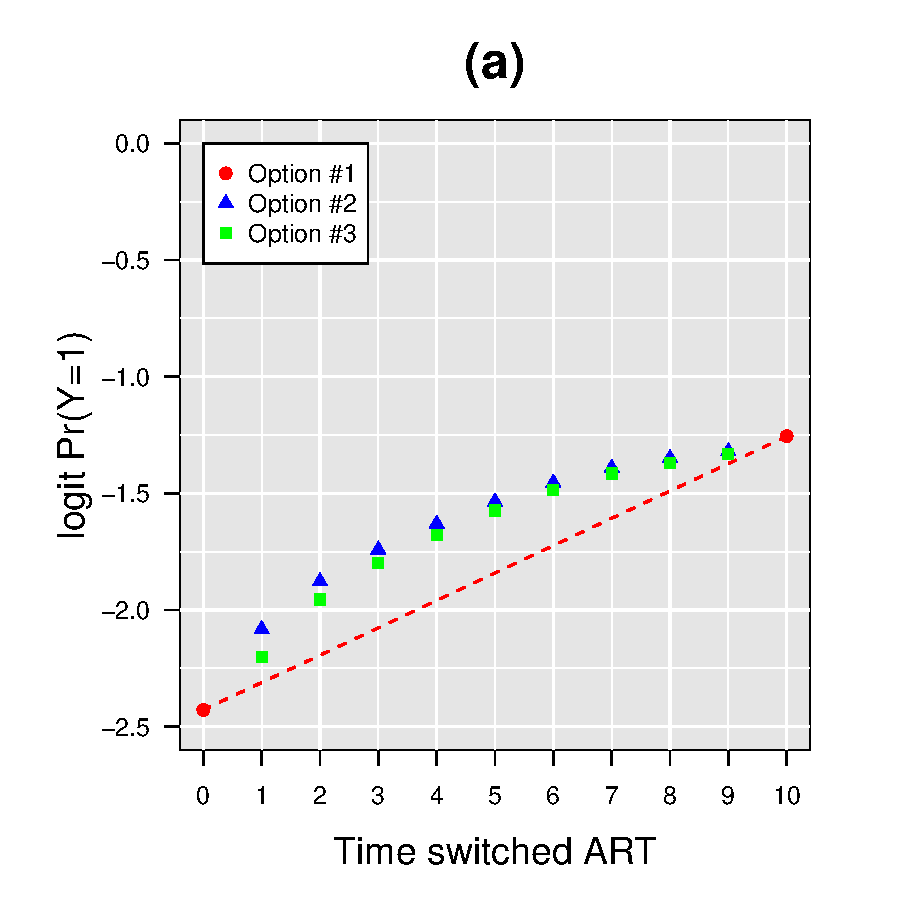
\includegraphics[width=3in]{truePsi_ZaffectsY} 
    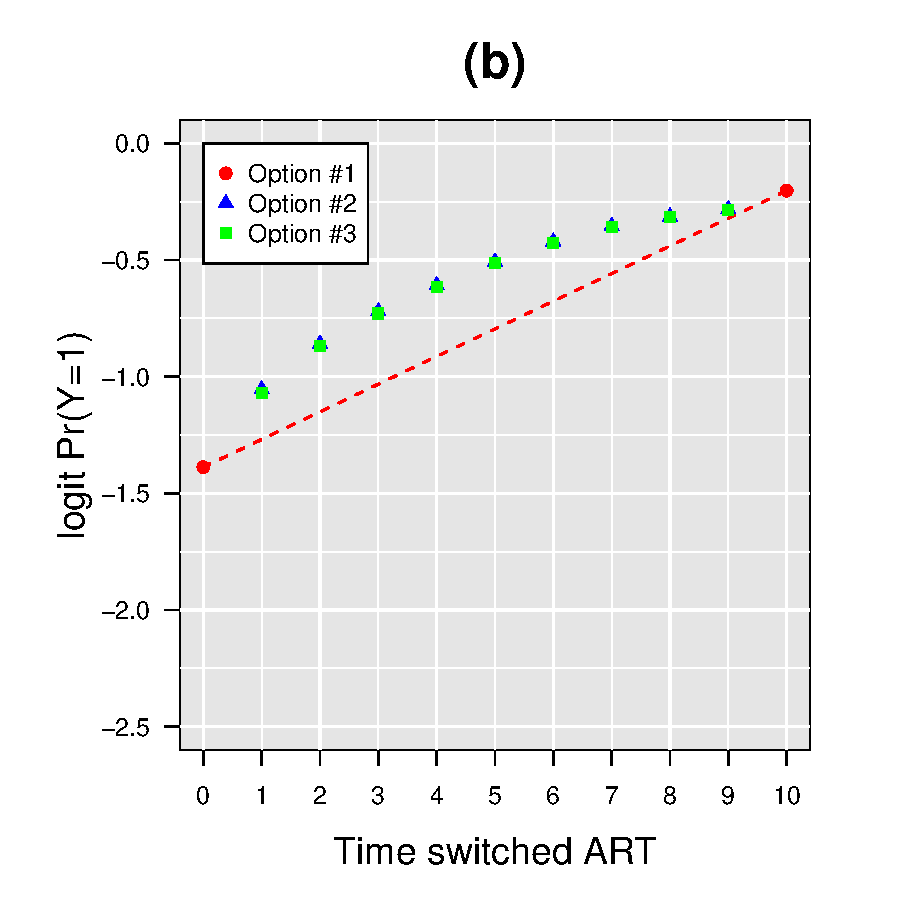
\includegraphics[width=3in]{truePsi_noZaffectsY} 
    \caption{True parameter values with (a) $\beta_Z=1.25$ and (b)
    $\beta_Z=0$ in the log-odds scale.}
    \label{fig:parms}
\end{figure}


%%%%%%%%%%%%%%%%%%%%%%%%%%%%%%%%%%%%%%%%%%%%%%%%%%%%%%%%%%%%%%%%%%%%%%%%%%%%%%%
%%%%%%%%%%%%%%%%%%%%%%%%%%%%%%%%%% RESULTS %%%%%%%%%%%%%%%%%%%%%%%%%%%%%%%%%%%%
%%%%%%%%%%%%%%%%%%%%%%%%%%%%%%%%%%%%%%%%%%%%%%%%%%%%%%%%%%%%%%%%%%%%%%%%%%%%%%%
\section{Results}

Discuss simulation results.


%%%%%%%%%%%%%%%%%%%%%%%%%%%%%%%%%%%%%%%%%%%%%%%%%%%%%%%%%%%%%%%%%%%%%%%%%%%%%%%
%%%%%%%%%%%%%%%%%%%%%%%%%%%%%%%%% DISCUSSION %%%%%%%%%%%%%%%%%%%%%%%%%%%%%%%%%%
%%%%%%%%%%%%%%%%%%%%%%%%%%%%%%%%%%%%%%%%%%%%%%%%%%%%%%%%%%%%%%%%%%%%%%%%%%%%%%%
\section{Discussion}

Discuss what we just did and implications.


%%%%%%%%%%%%%%%%%%%%%%%%%%%%%%%%%%%%%%%%%%%%%%%%%%%%%%%%%%%%%%%%%%%%%%%%%%%%%%%
%%%%%%%%%%%%%%%%%%%%%%%%%%%%%%%%% REFERENCES %%%%%%%%%%%%%%%%%%%%%%%%%%%%%%%%%%
%%%%%%%%%%%%%%%%%%%%%%%%%%%%%%%%%%%%%%%%%%%%%%%%%%%%%%%%%%%%%%%%%%%%%%%%%%%%%%%
%\clearpage
%\bibliography{/Users/tranlm/Dropbox/Bibtex/library}
%\bibliographystyle{abbrvnat}


\end{document}
